\documentclass[conference]{IEEEtran}
\IEEEoverridecommandlockouts
% The preceding line is only needed to identify funding in the first footnote. If that is unneeded, please comment it out.
\usepackage{cite}
\usepackage{amsmath,amssymb,amsfonts}
\usepackage{algorithmic}
\usepackage{graphicx}
\usepackage{textcomp}
\usepackage{xcolor}
\def\BibTeX{{\rm B\kern-.05em{\sc i\kern-.025em b}\kern-.08em
    T\kern-.1667em\lower.7ex\hbox{E}\kern-.125emX}}
\begin{document}

\title{Fall Detection in Video Sequences\\ Based on a Three-Stream Convolutional\\ Neural Network}

% \author{\IEEEauthorblockN{1\textsuperscript{st} Given Name Surname}
% \IEEEauthorblockA{\textit{dept. name of organization (of Aff.)} \\
% \textit{name of organization (of Aff.)}\\
% City, Country \\
% email address}}

\maketitle

\begin{abstract}
With falls being at the same time more susceptible in advanced ages and the second most common cause of accidental death to elders, detecting falls became a crucial research topic to an aging population~\cite{who2007report}. To this effect, we propose and evaluate the employment of a multi-stream approach to detect fall events. Three features (optical flow, saliency map, and RGB data) fed to each stream of a VGG-16 and classified by an SVM of whether there was or not a fall event. Experiments are conducted on two datasets, URFD and FDD, achieving accuracy rates of 98.84\% and 99.51\%, respectively, which outperforms the majority of the reviewed solutions.
\end{abstract}

\begin{IEEEkeywords}
Fall detection, multi-stream neural networks, optical flow, saliency, video, deep learning
\end{IEEEkeywords}

\section{Introduction}
With deteriorating health in advanced ages, even a minor fall can trigger a chain reaction of serious psychological and physical injuries to the elder population. Hence, the motivation for ambient assistant living solutions to both avoids falling from occurring and reducing the interval between a fall and help arrival.\par
The studies that detect falls as soon as they happen can be split into two main categories: hardware reliant solutions and vision based ones. The first one, which uses devices such as accelerometers and IMUs, has a satisfactory performance but are met with frustration from the subjects, mainly towards forgetting to use the device. Vision-based solutions, which allied to machine learning techniques, have shown promising results and, furthermore, do not rely on the subject wearing it.\par
Throughout the fall detection literature, techniques vary from threshold activation based, such as Sase et al.~\cite{sase2018human} detecting regions of interest after background subtraction, and a threshold activation function if the region of interest was under a third of the subject height in the frame. Bhandari et al.~\cite{bhandari2017novel} determined regions of interest via Shi-Tomasi, tracked them using Lucas-Kanade and set a threshold on the region of interest's speed and motion and also Albawendi et al.~\cite{albawendi2018video} who used a threshold activation on a silhouette shape. Another commonly used classification technique is the support vector machine (SVM), used by Harrou et al.~\cite{harrou2017vision}, that fed a feature extractor with the subject segmented from the frame. They compared extractor output with a multivariate exponentially-weighted moving average (MEWMA) and classified by an SVM. Panahi et al.~\cite{panahi2018human} subtracted the background from depth images, fitted an ellipse in the subject's shape, and classified it with SVM. Abobakr et al.~\cite{abobakr2017skeleton} also subtracted the background from depth images, applied a random decision forest to estimate the subject's posture, and an SVM to classify it. Regarding the subject's privacy, both Edgcomb et al.~\cite{edgcomb2012automated} and Lin et al.~\cite{lin2013fall} investigated privacy-prone features, such as blurring, silhouetting, and covering the body with shapes. Lu et al.~\cite{lu2018deep} employed a 3D convolutional neural network (CNN) followed by a long short-term memory (LSTM). Huang et al.~\cite{huang2018video} extracted the human pose with OpenPose and classified it with a VGG-16 architecture. Núñez-Marcos et al.~\cite{nunez2017vision} extracted the dense optical flow (OF) and also served it to a VGG-16. Anishchenko et al.~\cite{anishchenko2018machine} employed a modified AlexNet as a classifier. A few different approaches were also reported, such as K-nearest neighbor classifiers by Sehairi et al.~\cite{sehairi2018elderly} and Kwolek et al.~\cite{kwolek2015improving}. Hidden Markov model by Zerrouki et al.~\cite{zerrouki2018combined} and Qian et al.~\cite{qian2017recognizing}. Particle filtering by Yu et al.~\cite{yu2009fall}, Gaussian models by Yu et al.~\cite{yu2010robust} and Rougier et al.~\cite{rougier2011robust}. Furthermore, Xu et al.~\cite{xu2018new} produced a survey on fall detections systems.\par
The main contribution of this work is the development and evaluation of handcrafted features in a multi-stream learning model. We compare the effectiveness of three features extracted from videos frames: (i) optical flow, (ii) saliency map, and (iii) RGB data. These features are fed to a three-stream VGG-16 architecture, and their results compared with the literature.\par
We organized this paper as follows. In Section~\ref{sec:method}, we detail the proposed three-stream methodology for fall detection. In Section~\ref{sec:experiments}, we performed experiments and compared their results to other approaches available in the literature. Finally, in Section~\ref{sec:conclusion}, we conclude the work and suggest directions for future work.

\section{Background}
\label{background}

In this section, we describe some relevant concepts related to the topic under investigations and employed in Section~\ref{sec:method}.

\subsection{Optical Flow}
\label{sec:opticalflow}

\begin{figure*}[htbp]
\centerline{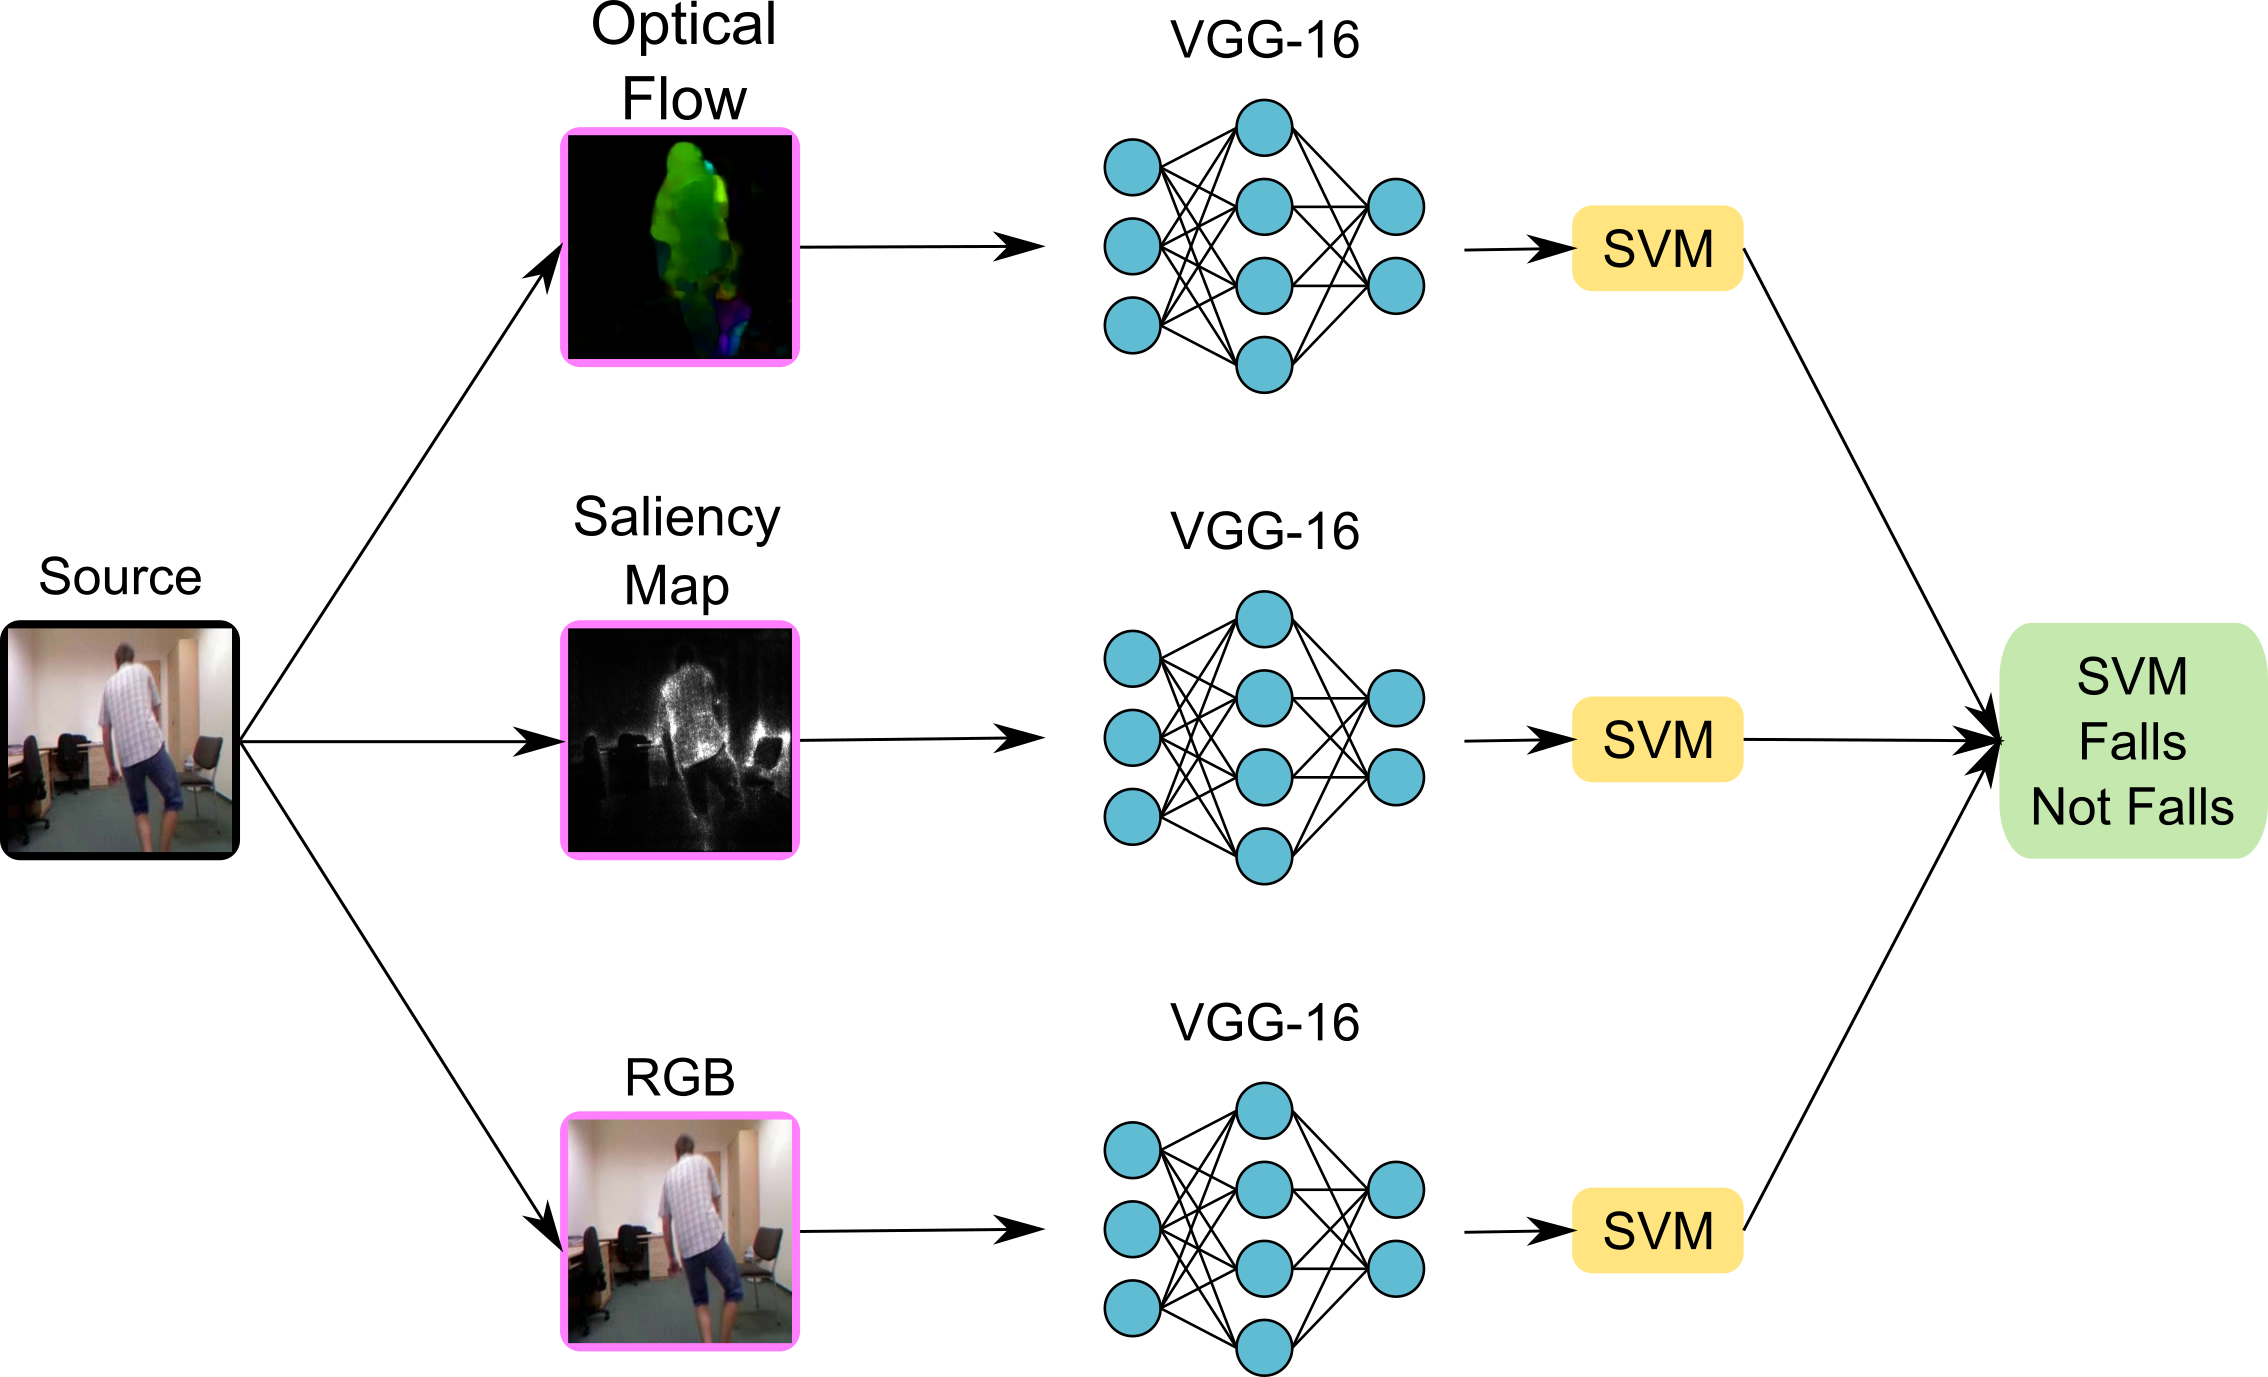
\includegraphics[width=0.57\linewidth]{figures/overview.png}}
\caption{Main components of the proposed fall detection method.}
\label{fig:overview}
\end{figure*}
Optical flow is a handcrafted feature that conveys movement information between two frames of a video, either by object or camera movement. Its ability to describe movement enables this feature to support the temporal aspect of a fall event in a deep network.\par
The extraction process considers a video frame as $I$ and $I(x, y, t)$ a pixel in this frame. Another frame collected $dt$ time later, and the distance that the same pixel moved $(dx, dy)$ is described in Equation~\ref{eq:of-dist}.
\begin{equation}
\label{eq:of-dist}
I(x, y, t)=I(x+dx, y+dy, t+dt)
\end{equation}
Equation~\ref{eq:of} is formed after applying a Taylor series approximation of right-hand side and dividing by $dt$, $f_t$ is the gradient given time, $f_x$ , $f_y$ , $u$, and $v$ are given in Equation~\ref{eq:of-grad}. Values of $u$ and $v$ can be achieved by different methods, such as the classical Lucas-Kanade~\cite{jain2018abnormal} or the one used in this work: Gunnar-Farnebäck~\cite{lowhur2015dense}.
\begin{equation}
\label{eq:of}
f_xu + f_yv + f_t=0
\end{equation}
\begin{equation}
\label{eq:of-grad}
f_x = \frac{\partial f}{\partial x}; \quad f_y = \frac{\partial f}{\partial y}u = \frac{\partial x}{\partial t}; \quad v = \frac{\partial y}{\partial t}
\end{equation}

\subsection{Saliency Map}
\label{sec:saliency}

Saliency map is envisioned as a visualizing technique to understand the learning process behind a deep network. Its extraction can occur in many ways, one of those being the practice of feeding an image $I$ and its class label $c$ to the network, then, freezing the weights on the network and compute the gradients of $c$ to the pixels of $I$. Consider $S_c(I)$ to be the class score function for an image $I$ and, for this simple explanation, that it is a simple linear function, $S_c(I) = w_c^T + b_c$. With $w$ being the weights of the network and $b$ the bias, it is possible to notice that the magnitude of elements of $w$ affects the importance of the corresponding pixels in $I$ with class $c$.\par
The choice of saliency map as a stream is due to its spatial relation to the frame, as the raw RGB frames are prone to environmental interference, and its performance in the works developed by Zuo et al.~\cite{zuo2019enhanced} and Meng et al.~\cite{Meng2018interpretable}. In our work, we applied the saliency method described by Sundararajan et al.~\cite{sundararajan2017axiomatic}.

\section{Fall Detection Method}
\label{sec:method}

As further detailed in the following subsections, we used an ensemble of VGG-16s to classify between fall and not fall in video sequences. Figure~\ref{fig:overview} illustrates an overview of the proposed method.

\subsection{Transfer Learning}

The selected datasets, further detailed in Section~\ref{sec:experiments}, possess relatively few human fall samples in their videos, which would limit the CNNs learning capabilities to detect fall events. Hence, the importance of transfer learning.\par
The first 14 layers of the VGG-16 architecture were trained on the ImageNet~\cite{imagenet_cvpr09} dataset and, later on, these same layers were fine-tuned over the UCF101~\cite{soomro2012ucf101} dataset. The reasoning being that the network would initially learn low-level features from the ImageNet classes, and focus these features on human activities with the UCF101 videos, Figure~\ref{fig:pre14}. Núñez-Marcos et al.~\cite{nunez2017vision} executed this step and released their weight files publicly.\par
\begin{figure}[htbp]
\centerline{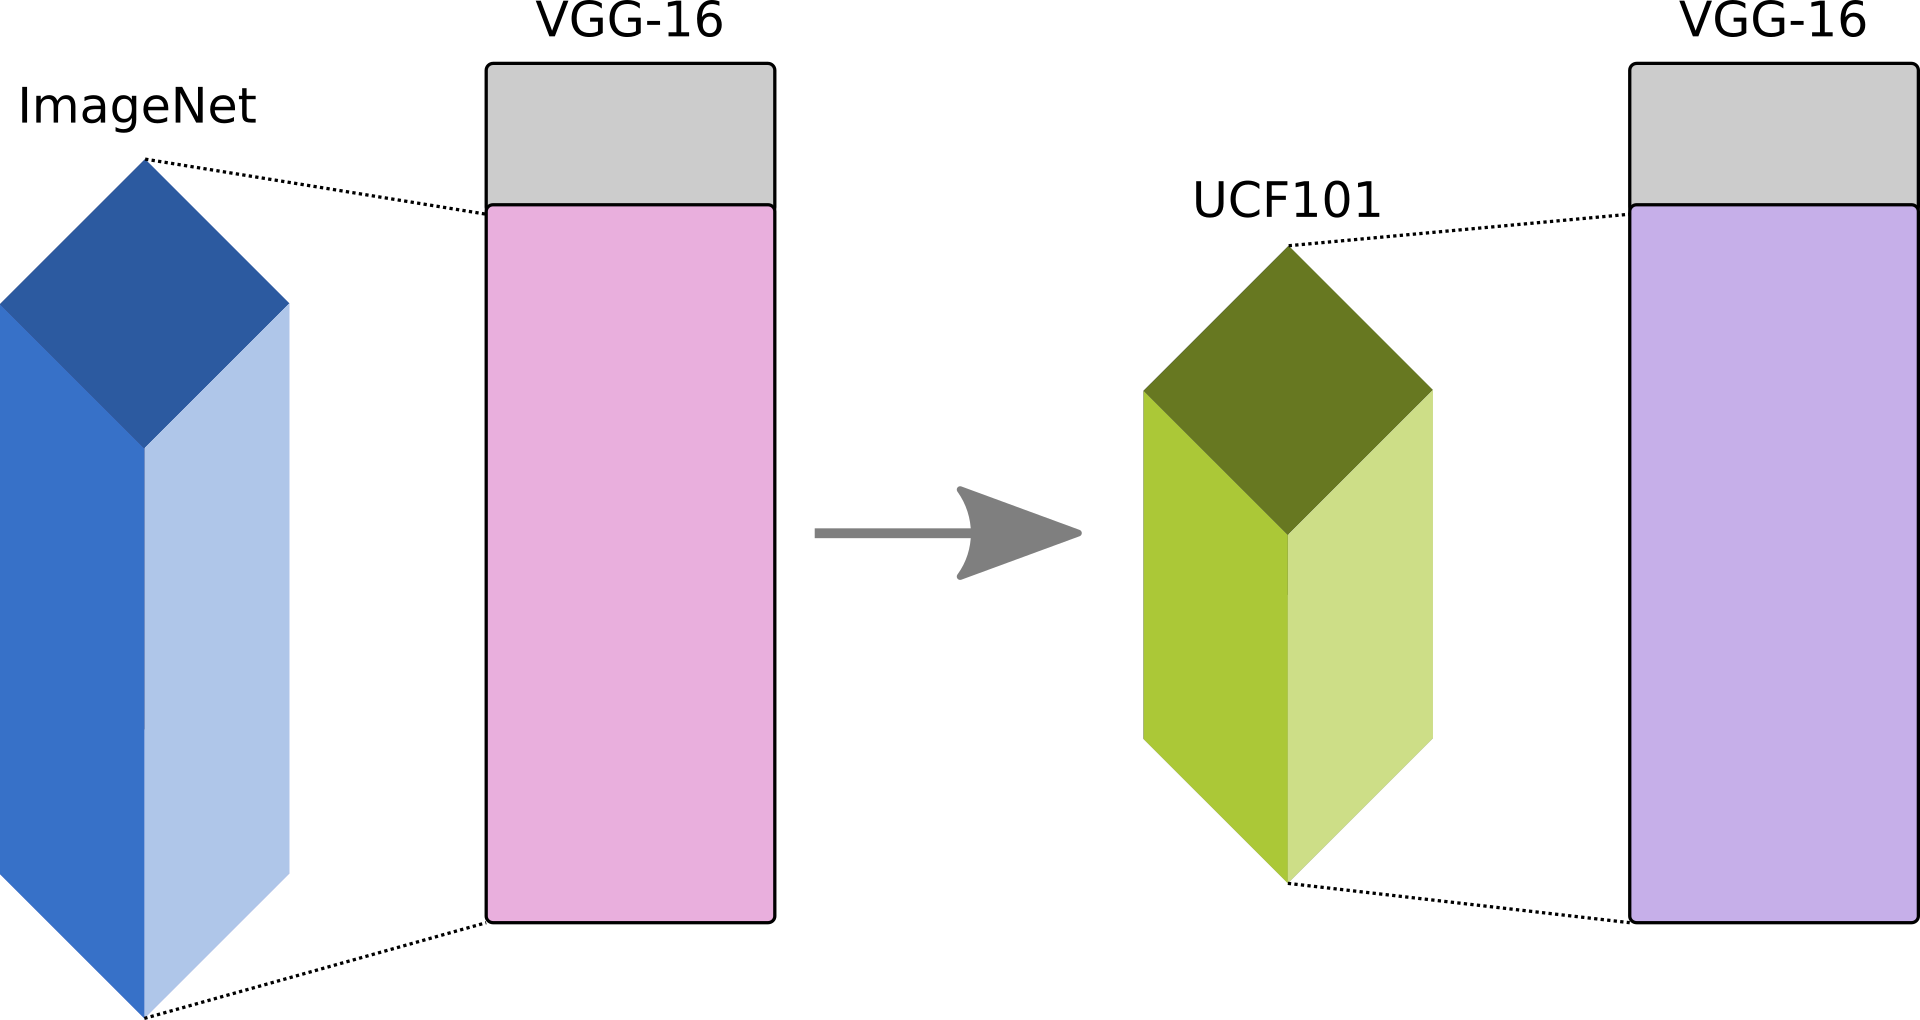
\includegraphics[width=0.9\linewidth]{figures/pre14.png}}
\caption{Deep layers being trained on ImagetNet and UCF101.}
\label{fig:pre14}
\end{figure}
We froze the 14 initial layer's weights and fine-tuned the
last two fully connected layers were fine-tuned, with dropout
regularization. Each stream executed this last fine-tuning step,
totaling three executions (Figure~\ref{fig:pos14}).
\begin{figure}[htbp]
\centerline{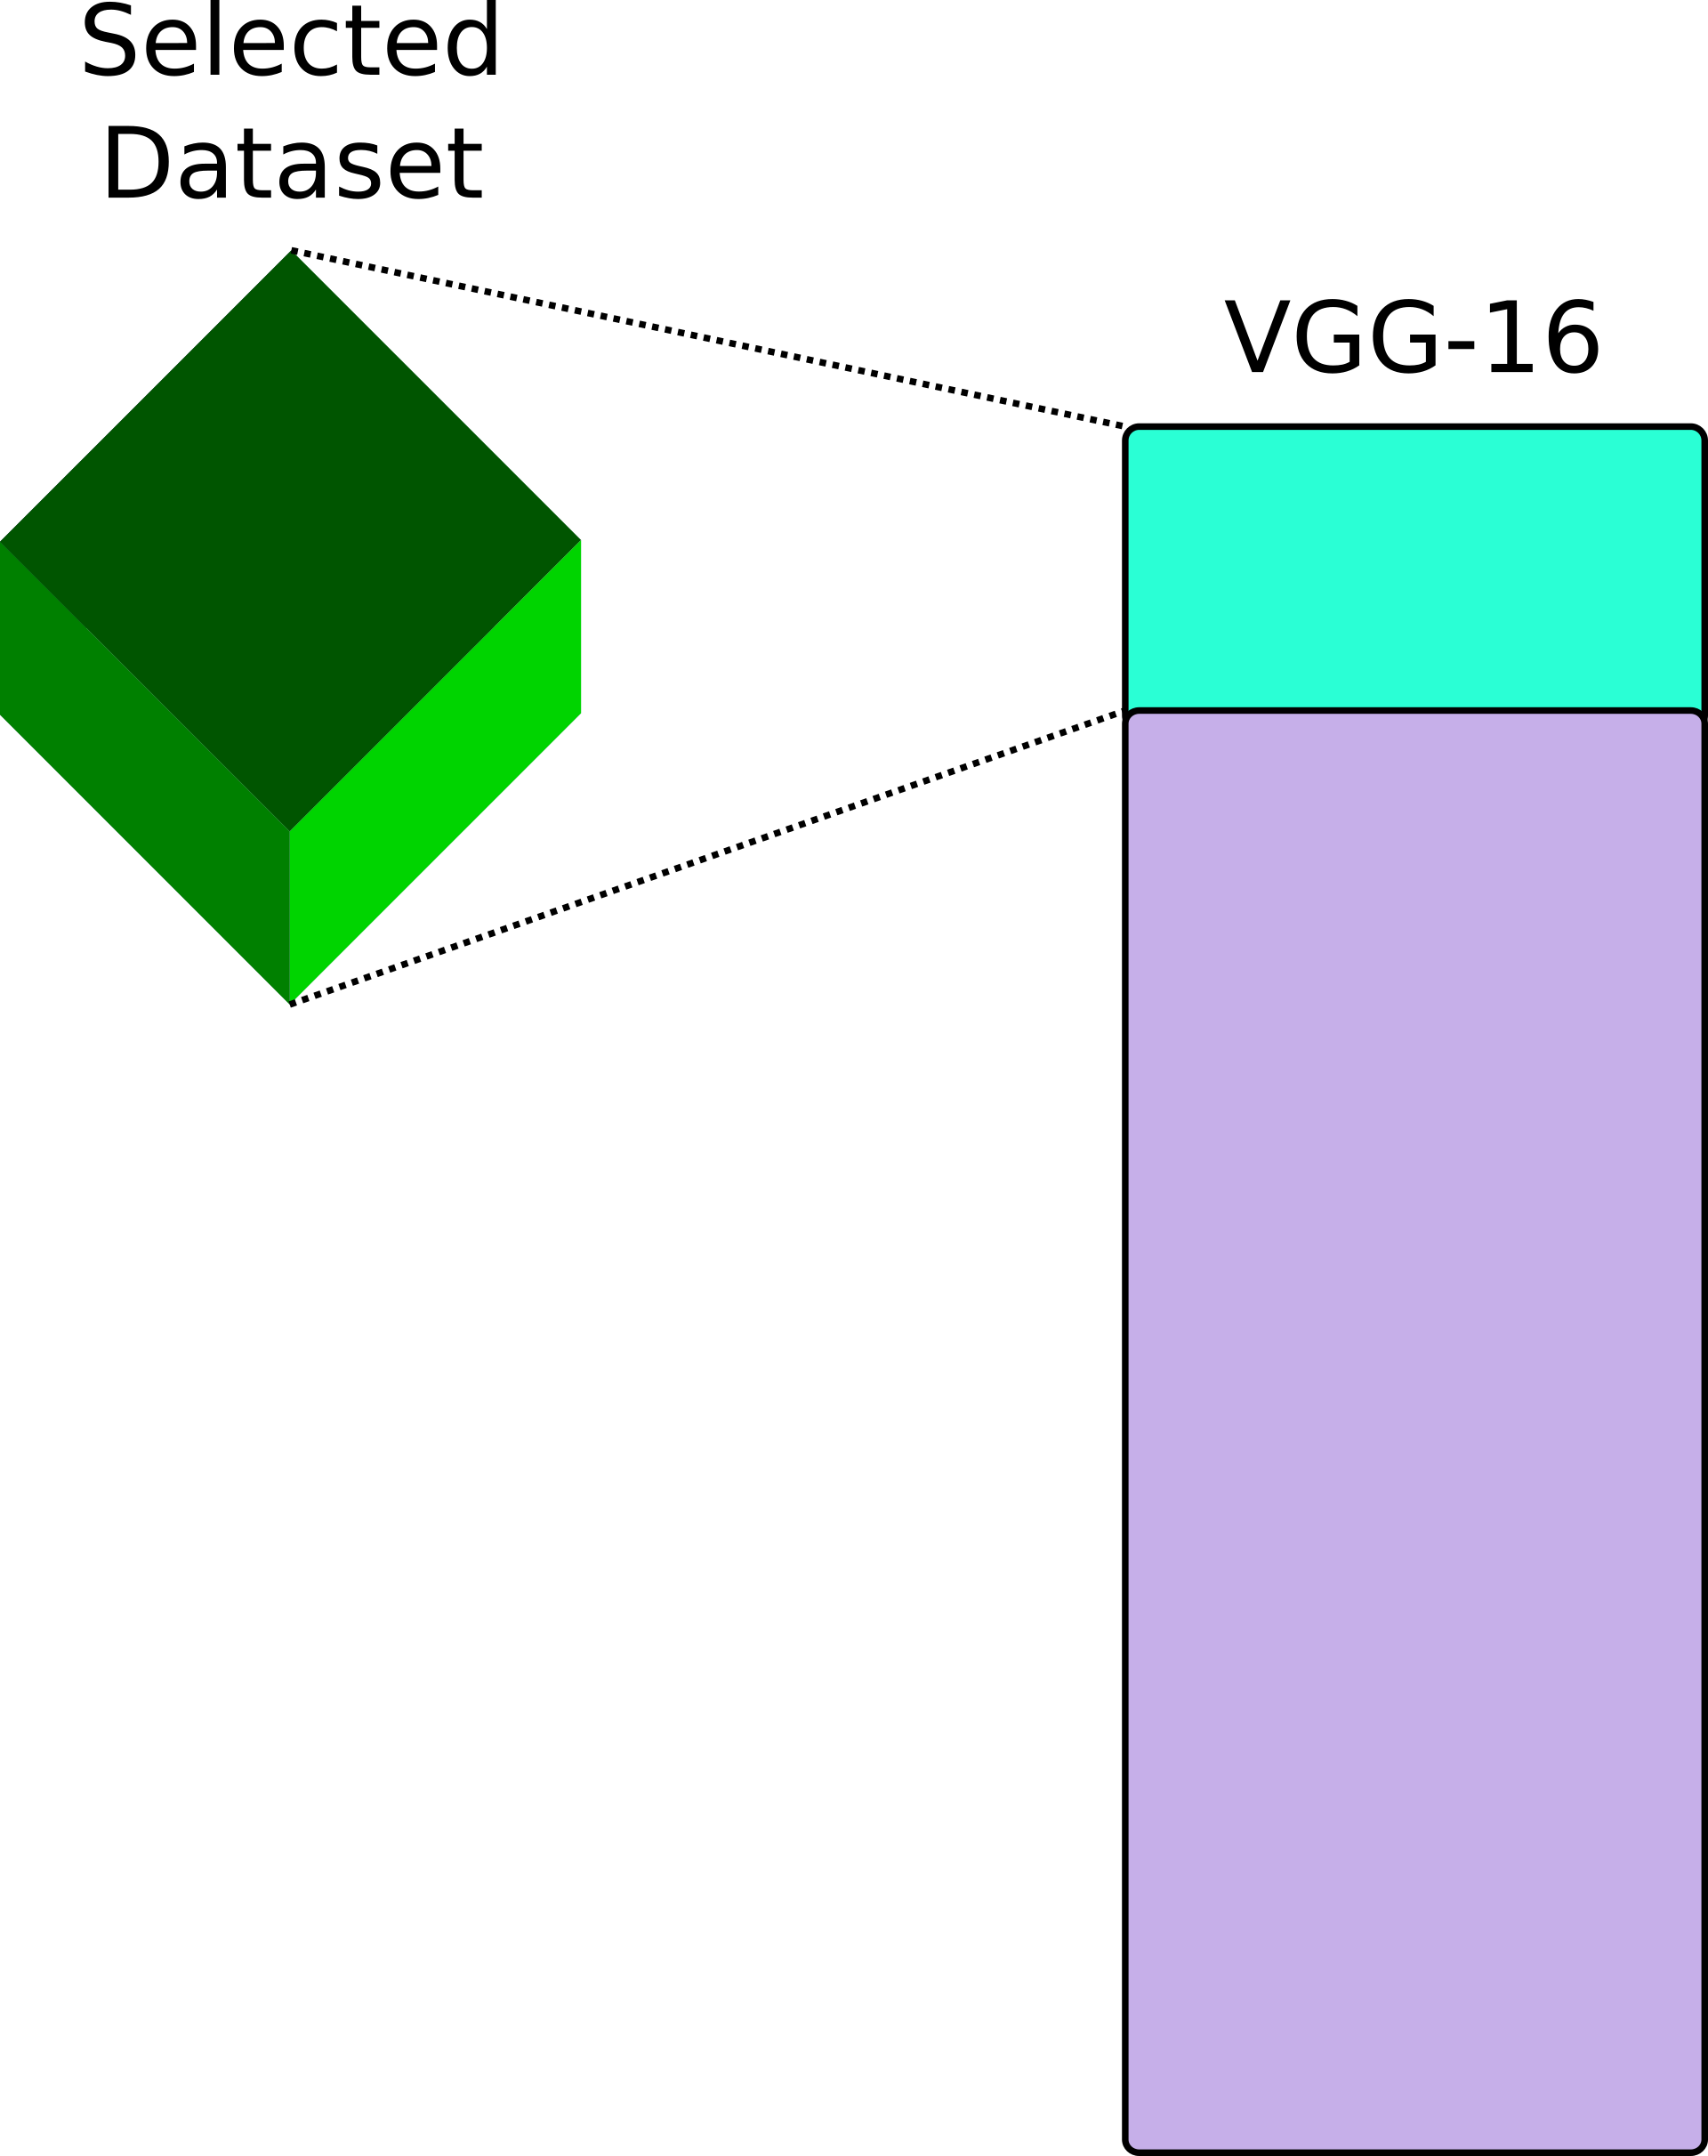
\includegraphics[width=0.4\linewidth]{figures/pos14.png}}
\caption{Fully connected layers training.}
\label{fig:pos14}
\end{figure}

\subsection{Classification}
\label{sec:classification}

Wang et al.~\cite{wang2015towards} reported that networks employing multi-stream classifiers outperformed their single-streamed peers. Inspired on this finding, an SVM classifier fed with the outputs of each stream, vectors between 0 and 1, generates a ($x$, $y$, $z$) vector. A second SVM uses this vector to classify between fall and not fall (Figure~\ref{fig:overview}).

\subsection{Streams Input}

The optical flow and saliency map features were fed to the streams, explained in Subsection~\ref{sec:classification}. Furthermore, given the neural networks capability of learning relevant features to describe their input, the RGB frame itself was fed to the third stream.
\paragraph{Optical Flow} represents the temporal relation between frames and to fully gather this property it was used as a stack of optical flows on top of a sliding window of frames, as suggested by Núñez-Marcos et al.~\cite{nunez2017vision}. The sliding window has a size of $L$ frames and gathers 2$L$ components ($L$ horizontal ($d_t^x$) + $L$ vertical ($d_t^y$) optical flow component vector fields) creating a stack $O$ = \{$d_t^x$, $d_t^y$, $d_{t+1}^x$, $d_{t+1}^y$, ..., $d_{t+L}^x$, $d_{t+L}^y$ \}. The total number of stacks is given by $N$-$L$+$1$, where $N$ is the number of frames in a video. Figure~\ref{fig:of} shows an extracted example.
\begin{figure}[htbp]
\centerline{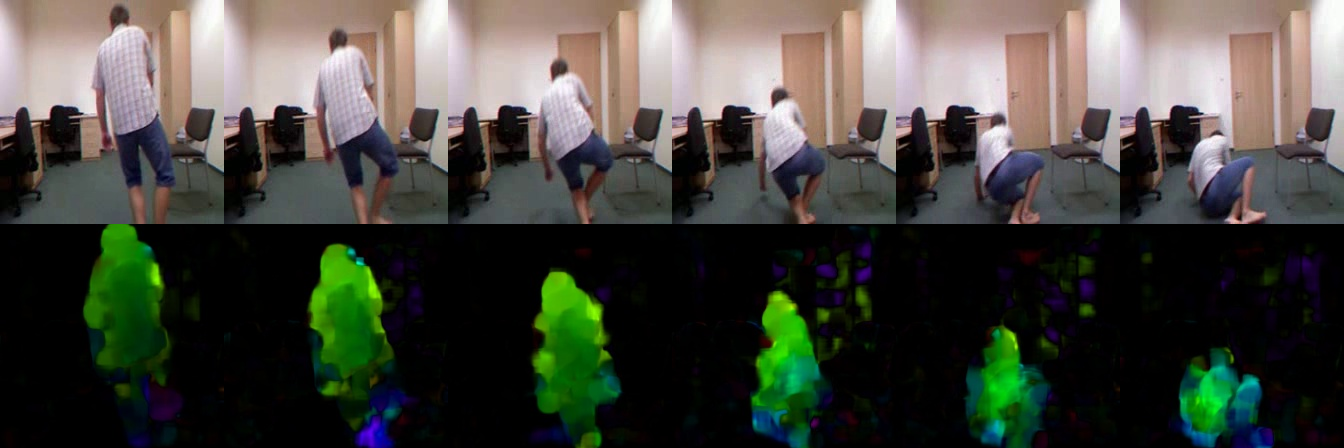
\includegraphics[width=\linewidth]{figures/of.png}}
\caption{A frame and its extracted optical flow.}
\label{fig:of}
\end{figure}
\paragraph{Saliency Map} is composed of pixels varying from 0 to 1, and was fed as a gray-scale image to the network. Figure~\ref{fig:sal} shows and extracted example.
\begin{figure}[htbp]
\centerline{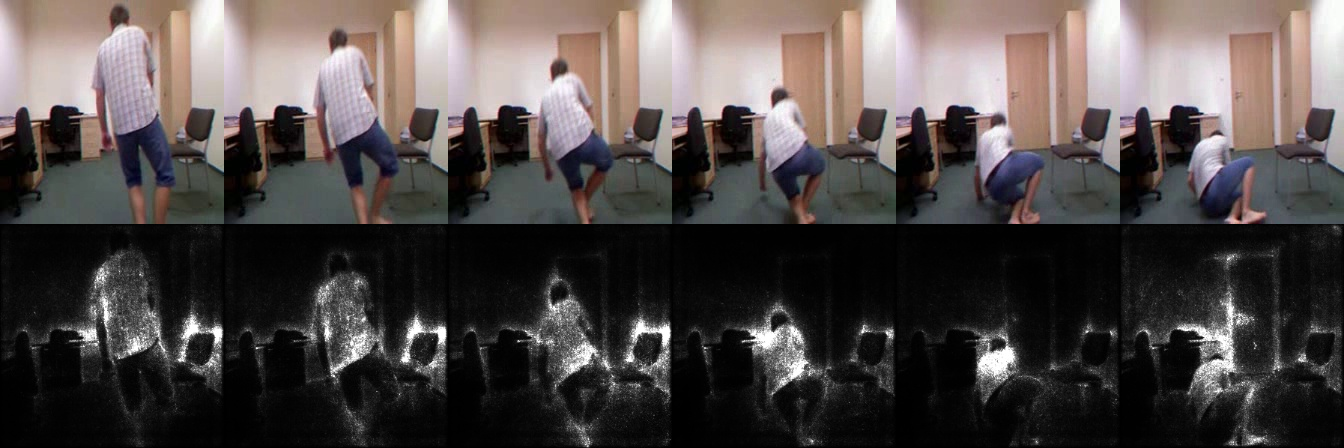
\includegraphics[width=\linewidth]{figures/sal.png}}
\caption{A frame and its extracted saliency map.}
\label{fig:sal}
\end{figure}

\section{Experiments}
\label{sec:experiments}

Our experiments were performed on two publicly available
datasets: URFD~\cite{kepski2014human} and FDD~\cite{charfi2013optimised}.\par
The URFD dataset contains 70 videos: (i) 30 videos of falls; and (ii) 40 videos of daily living activities, recorded from a top-down and front view perspective by two Microsoft Kinect cameras. Each frame is labeled in three categories: if the person is lying on the ground, not lying on the ground, and in an intermediate pose.\par
The FDD dataset is composed of 191 videos, of which 143 are falls, recorded from a surveillance camera perspective by a single RGB camera. With every frame annotated between fall and not fall.\par
To enable a comparison with other works, we evaluated our method through three metrics: (i) sensitivity, which reflects the true positive rate; (ii) specificity, also known as the true negative rate; and (iii) accuracy, which represents the overall performance of the method.\par
We used a learning rate of $10^{−4}$ , 500 epochs, 5-fold cross-validation, mini-batches of $2^{10}$ , and Adam optimization. We also experimented with different classes and weights, however, further tuning of the hyper-parameters we were able to keep both classes on the same weight. As explained in Section~\ref{sec:classification}, a double SVM is used to ensemble the outputs.\par
Tables~\ref{tab:urfd-ensem} and~\ref{tab:urfd-our-their} show the results obtained on the URFD dataset. In Table~\ref{tab:urfd-ensem}, we compare each single-stream feature with their multi-stream counterpart. The optical flow single-stream acquired the highest accuracy, at 97.57\%, and the multi-stream was still able to outperform it, at 98.84\%. Table~\ref{tab:urfd-our-their} compares our result with other works in the literature, whilst not all works measured their sensitivity and specificity, all of them reported their accuracy.\par
The accuracy and specificity of our method performed better than most and kept the same 100\% sensitivity. The approach developed by Lu et al.~\cite{lu2018deep} was the only work that outperformed ours. We conjecture that the reason for such is the temporal importance to detect a fall event, and their usage of LSTM would better cater this relationship.\par
Tables~\ref{tab:fdd-ensem} and~\ref{tab:fdd-our-their} report the results extracted from the FDD dataset. Homologous to the URFD report, Table~\ref{tab:fdd-ensem} compares each single-stream with the multi-stream approach. The multi-stream achieved 99.51\% accuracy, and the highest single-stream score was again the optical flow, with 99.11\%. When comparing our results against the literature, in Table~\ref{tab:fdd-our-their}, ours outperformed every other one, regarding accuracy and sensitivity. It was 0.05\% worse than Charfi et al.'s~\cite{charfi2013optimised} specificity. Our results also confirmed the findings of Wang et al.~\cite{wang2015towards} since each feature stream did not perform great on their own, however, when applied together, they contributed to the state-of-the-art results towards fall detection.
\begin{table*}[]
\centering
\caption{Results on URFD dataset for single-stream \textit{vs} multi-stream (descending order of accuracy).}
\label{tab:urfd-ensem}
\begin{tabular}{llcccl}
\hline
 &  & Sensitivity (\%) & Specificity (\%) & Accuracy (\%) &  \\ \hline
 & OF + RGB + Sal & \textbf{100} & \textbf{98.77} & \textbf{98.84} &  \\
 & Optical Flow & \textbf{100} & 97.42 & 97.57 &  \\
 & RGB & \textbf{100} & 96.35 & 96.56 &  \\
 & Saliency & 93.67 & 93.39 & 93.40 &  \\ \hline
\end{tabular}
\end{table*}
\begin{table*}[]
\centering
\caption{Comparison of the results on URFD datasets (descending order of accuracy).}
\label{tab:urfd-our-their}
\begin{tabular}{llcccl}
\hline
 &                                                      & Sensitivity (\%)  & Specificity (\%)  & Accuracy (\%)     & \\ \hline
 & Lu et al.~\cite{lu2018deep}                          & -                 & -                 & \textbf{99.27}    & \\
 & Ours                                                 & \textbf{100}      & \textbf{98.77}    & 98.84             & \\
 & Carneiro et al.~\cite{carneiro2019multi}                                                 & \textbf{100}      & \textbf{98.61}    & 98.77             & \\
 & Panahi et al.~\cite{panahi2018human}                 & 97.05             & 97.02             & 97.14             & \\
 & Zerrouki and Houacine~\cite{zerrouki2018combined}    & -                 & -                 & 96.88             & \\
 & Harrou et al.~\cite{harrou2017vision}                & -                 & -                 & 96.66             & \\
 & Abobakr et al.~\cite{abobakr2017skeleton}            & \textbf{100}      & 0.91              & 96.00             & \\
 & Bhandari et al.~\cite{bhandari2017novel}             & 96.66             & -                 & 95.71             & \\
 & Kwolek and Kepski~\cite{kwolek2015improving}         & \textbf{100}      & 92.50             & 95.71             & \\
 & N\'u\~nez-Marcos et al.~\cite{nunez2017vision}       & \textbf{100}      & 92.00             & 95.00             & \\
 & Sase et al.~\cite{sase2018human}                     & 81.00             & -                 & 90.00             & \\ \hline
\end{tabular}
\end{table*}
\begin{table*}[]
\centering
\caption{Results on FDD dataset for single-stream \textit{vs} multi-stream (descending order of accuracy).}
\label{tab:fdd-ensem}
\begin{tabular}{llcccl}
\hline
 &  & Sensitivity (\%) & Specificity (\%) & Accuracy (\%) &  \\ \hline
 & OF + RGB + Sal & \textbf{99.43} & \textbf{99.55} & \textbf{99.51} &  \\
 & Optical Flow & 99.07             & 99.12             & 99.11             &  \\
 & RGB & 98.85             & 98.41             & 98.55             &  \\
 & Saliency & 88.39             & 92.40             & 91.25             & \\ \hline
\end{tabular}
\end{table*}
\begin{table*}[]
\centering
\caption{Comparison of the results on FDD dataset (descending order of accuracy).}
\label{tab:fdd-our-their}
\begin{tabular}{llcccl}
\hline
 &                                                      & Sensitivity (\%)  & Specificity (\%)  & Accuracy (\%)     & \\ \hline
 & Ours                                                 & \textbf{99.43}    & 99.55             & \textbf{99.51}    & \\
 & Lu et al.~\cite{lu2018deep}                          & -                 & -                 & 99.36             & \\
 & Sehairi et al.~\cite{sehairi2018elderly}             & -                 & -                 & 98.91             & \\
 & Carneiro et al.~\cite{carneiro2019multi}                                                 & \textbf{99.9}      & \textbf{98.32}    & 98.43             & \\
 & Zerrouki and Houacine~\cite{zerrouki2018combined}    & -                 & -                 & 97.02             & \\
 & Harrou et al.~\cite{harrou2017vision}                & -                 & -                 & 97.02             & \\
 & Charfi et al.~\cite{charfi2012definition}            & 98.0              & \textbf{99.60}    & -                 & \\
 & N\'u\~nez-Marcos et al.~\cite{nunez2017vision}       & 99.0              & 97.00             & 97.00             & \\ \hline
\end{tabular}
\end{table*}
 
\section{Conclusion and Future Work}
\label{sec:conclusion}

In this paper, we proposed a method to detect human fall events, based on the employment of a multi-stream convolutional neural network. Each stream was served an extracted feature, as follows: (i) optical flow, (ii) saliency map, and (iii) the RGB frame itself. The double SVM performed the ensemble approach. The proposed method was evaluated on the RFD and FDD datasets. Our solution outperformed the related literature in most cases, indicating that multi-stream approaches and the selected features can be useful to detect human fall events.\par
It is worth discussing the selected features and some literature results. As et al.~\cite{chernbumroong2012elderly} noticed that privacy concerns might arise on video-based approaches, the selected features can conceal one's identity. Despite their feature performance, both optical flow and saliency map are timely and computationally intensive to extract, which would halt their implementation in a real-time system.\par
Considering the goal of this work in exploring features to the fall detection problem, it is relevant to weight their extraction process against their results. Regarding other works in the literature, some seemed to dismiss the importance of the sensitivity metric, which quantifies the avoidance of false negatives. A World Health Organization report~\cite{who2007report} enlightens the severity of an elderly fall, thus the importance of a high sensitivity metric.\par
From the results reported in Tables~\ref{tab:urfd-our-their} and~\ref{tab:fdd-our-their}, it is possible to observe a saturation of these datasets, and as also reported by Chernbumroong et al.~\cite{chernbumroong2012elderly}, systems trained on artificial environments did not perform as well on real-life scenarios. Therefore, since it is important to come up with a more extensive dataset that better resembles the actual application setup, Mastorakis et al.~\cite{mastorakis2018fall} published a simulated dataset of fall events. Cheaper features and deep networks for generating comparable results could also be explored.

\section*{Acknowledgment}

Omitted for blind review.

%\begin{thebibliography}{00}
%\end{thebibliography}

\bibliographystyle{IEEEtran}
\bibliography{paper}

\end{document}

%  3. Comments to authors

%     Fall Detection in Video Sequences Based on a Three-Stream Convolutional Neural Network


%     This paper proposes and evaluates the multi-stream approach for fall detection applications. Fall detection is an important and challenging application. This paper applies the standard technique used in action recognition for fall detection and shows strong results in two datasets URFD and FDD.

%     Pros:
%     The proposed approach gives decent results in two fall detection dataset.

%     The proposed multi-stream approach is technically sound, and I also appreciate the ablation study results.

%     Cons:
%     I think this paper does not address the cross-dataset problem. Ideally, it would be better to train the model on one or two scenarios but test on the other unseen situations. This evaluation helps to understand if the proposed approach can generalize well for practical use.

%     The other problem with the proposed approach is the lack of an important technical justification. It seems that the saliency map is an interesting attemp. But I am wondering why there is no evaluation on the foreground subtraction, which appears to be more common than the saliency map.

%     Regarding the technical choice, I think SVM with the pre-trained imagenet features is a bit out of the dated technique. The current action recognition technique often involves end-to-end training, which would be useful to evaluate.

%     I concern the metrics used in this paper too. Why is the only accuracy used? Ideally, precision and recall would be useful. In other action recognition papers, precision@1 and precision@5 are often used too.

% 3. Comments to authors

%     The authors propose a multi-stream method (optical flow, saliency map, RGB data) to detect fall events. Firstly, optical flow, saliency map, RGB data are extracted to fed a VGG-16, respectively. Then an SVM is used to classify whether there was a fall event. They demonstrate the efficacy of the proposed model on two datasets.

%     However, there are some questions.

%     # Why use SVM instead of direct neural network to supervise learning.

%     #Why use two SVMs, the features of three streams can be concatenated, and use an SVM to classify.

%  3. Comments to authors

%     In this paper, the authors proposed the use of a deep learning approach to detect fall events. In order to detect the falls, the authors came up with a set of handcrafted features and used in conjunction with VGG-16 architecture. A SVM is used as a final classification layer on top of the VGG-16 outputs. Finally, different sets of architectures are trained and compared in terms of performance.

%     Good Points:

%     1. The problem formulation and the motivation behind the proposed work is interesting. All the sections are well written with minimal grammatical errors.

%     2. A well described background on optical flow, saliency map and transfer learning.
%     Experimentation setup and hyperparameters are detailed in a very clear and transparent manner.

%     3. The proposed approach was experimented on two publicly available datasets and the results are compared properly compared against the other existing methods in the literature.

%     Comments to Address:

%     1. No theoretical evidence was provided regarding why SVM was used as the final classification layer. Have you tried adding a few extra concatenation layers at the end for merging the three networks instead of SVM, thereby resulting in a more efficient backpropagation?

%     2. It would be interesting to know if the authors have explored any other architectures instead of VGG-16, which might be more suitable for these features.

%     3. It would be better to add statistical test results in order to verify the statistical significance of the proposed method over the other methods.

%     Overall, I would recommend this paper as an accept, and the paper could be improved by adding a bit of theoretical evidence on the proposed work and describing about the pros and cons of the alternative approaches, and also by adding statistical significance results.